\chapter{Processus d'élaboration d'un référentiel}

\begin{figure}[h!]
    \begin{center}
        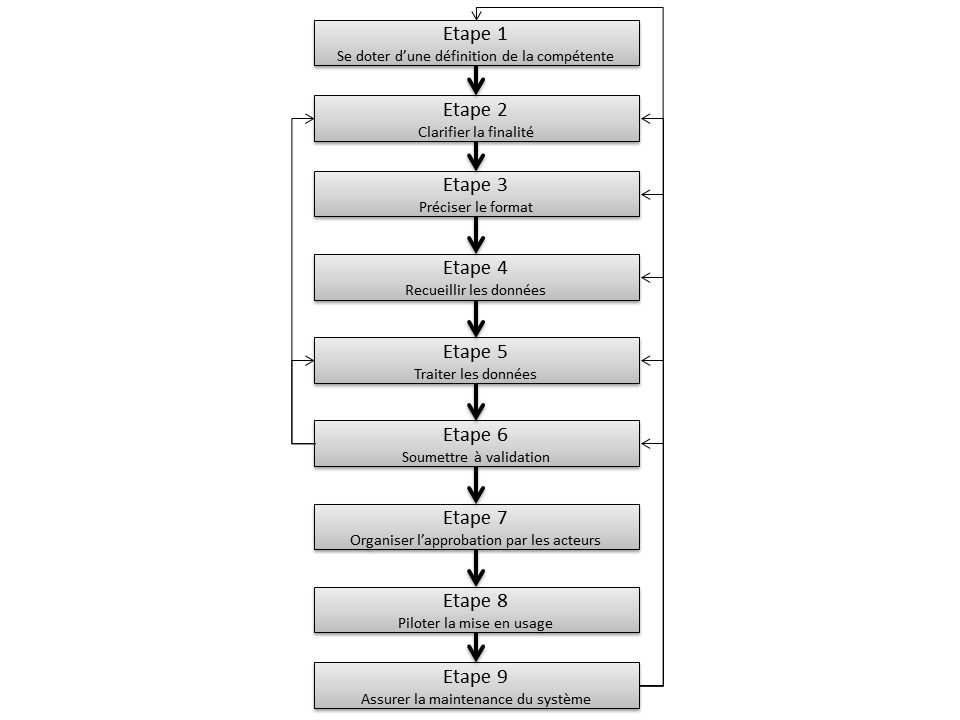
\includegraphics[scale=0.5]{document/process.png}
        \caption{Processus de l'élaboration et de la mise en service d'un référentiel de compétence. Source \citep[pp.41]{refcompetence} }
        \label{process}
    \end{center}
\end{figure}






\section{Définition des tâches}

\begin{description}
    \item[Support] 
    \item[Formation basique]
    \item[Formation avancée]
    \item[Formation web]
    \item[Développement Backend]
    \item[Développement Front end]
    
\end{description}

\subsection{Les tâches impliquée dans les projets clients}
\begin{description}
    \item[Analyse Technique, estimation et faisabilité] 
    \item[Développement Backend]
    \item[Création des vues]
    \item[Développement Front end]
    \item[Web Design]
    \item[Test fonctionnel]
    \item[Test automatique backend] -
    \item[Test automatique frontend] -
    \item[Revue de la qualité du code]
    \item[Intégration]
    \item[Documentation Technique]
    \item[Documentation Fonctionnelle]
    \item[Support] -
    \item[Version Migration]
    \item[Data Migration]
    \item[Odoo Deployement]
    \item[Administration Postgresql]
    \item[Performance optimisation] - 
    \item[Méthode agile]       -
    \item[Gestion des sources] -
\end{description}
